\section{Unary heterogeneous systems}

To start the approach to the thermodynamic study of material it's better to first approach simple systems, and in this field the simplest case that one can think of are \textbf{unary systems}. The latter are simply defined as systems where only one element is present, such as Carbon, Silicon or also more complicated ones such as water or \ce{SiO_2}. In fact, also system composed by molecules can be thought as unary as long as we work in a range where the smallest component is stable and no spontaneous dissociation appears.
\dfn{Unary systems}
{
    A system is sad to be unary if is composed by only one main component, which can be a molecule or an atom, that is stable inside the working range of the analysis.
}

\noindent
Our aim in working with this system is start to understand how they present themselves in nature in different ambient. Basically we will explain how to predict if a material at a certain pressure and temperature is in gases, solid or liquid state, comprehending how to read and construct a \textbf{phase diagram} for these simple cases.

For the readers that has never seen, or heard of, a phase diagram some examples for the cases of Carbon and Water are reported in \figref{fig:PhaseDia}.
\begin{figure}[b]
    \centering
    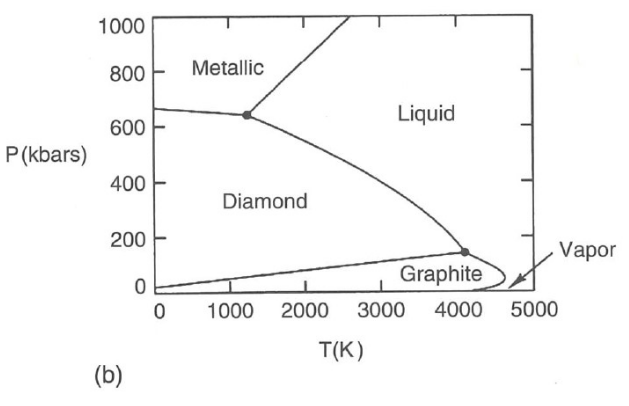
\includegraphics[width=0.43\textwidth]{Immagini/DiaCarb.png}
    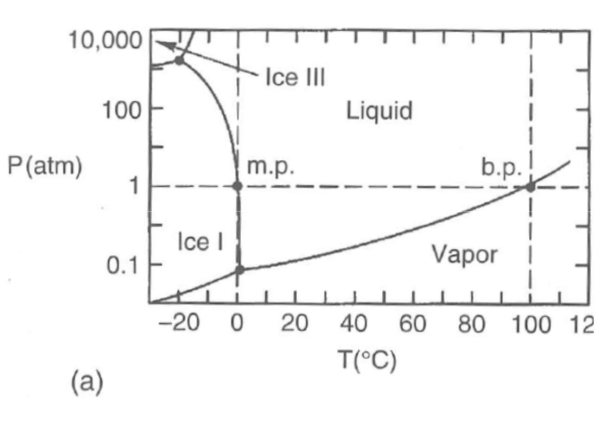
\includegraphics[width=0.4\textwidth]{Immagini/DiagraWater.png}
    \caption{
        Phase diagrams of simple unary systems: Carbon(a) and Water(b). Both are reported in a P vs T graph, where we can clearly see the triple points and the coexistence lines. 
    }
    \label{fig:PhaseDia}
\end{figure}
These type of plots are made to clearly show the state in which the material present itself in the selected region of phase space. In our case we selected the $(P, T)$ representation, where is possible to see at what pressure and temperature the two materials are in a solid state or transform to a liquid one etc. Nevertheless, the real points of interest inside the graph are the lines that marks the boundaries between phases. They are called \textbf{coexistence lines} and are a special subspace of phase space where both phases can coexist at equilibrium. A condition that allow us to model what happens in that region and predict their form and, therefore, the boundaries that describe the phase diagram. At last, of great interest are also the points at the intersection of two lines, called \textbf{triple points}, where three states of matter coexist at the same time, which we will see is the maximum number of state that can coexist in a unary system.

\subsection{Equilibrium conditions}

To draw a phase diagram of a system we need to predict the positions of the coexistence line, finding out the subset of phase space where two, or more, phase of matter are in equilibrium with each other and can, therefore, coexist. To do that is needless to say that we need to define what being in equilibrium means, and in particular finding out the physical conditions that tells us when two phases of matter are in equilibrium with each others. In order to do that simple thermodynamic considerations allow us to arrive to the following results.
\thm{Equilibrium conditions}
{
    Inside a unary system two phases $\alpha, \beta$ of matter can coexist at equilibrium, creating a heterogeneous system, only if the relation for \textbf{thermal}, \textbf{mechanical} and \textbf{chemical} equilibrium are satisfied, namely:
    \begin{equation}
        \label{eq:equiCond}
        T^\alpha = T^\beta, \hspace{2cm} P^\alpha = P^\beta, \hspace{2cm} \mu^\alpha = \mu^\beta.
    \end{equation}
}
\pf{Proof}
{
    Let's imagine to start with the system composed by $\alpha$ and $\beta$ being an open one inside an environment. After some time the studied system will evolve to an equilibrium state within the environment, which nevertheless will not depend on it. This is something that we can easily understand since, for the zeroth principle of thermodynamics, if we close the system when in equilibrium, basically eliminating the environment, the state of the $\alpha$ and $\beta$ unary system will remain untouched. Basically the evolution of the open system leads to an equilibrium situation that is analogues to the case of a closed one, meaning that at equilibrium we can consider $\alpha \cup \beta$ as closed having that the following conditions must be true
    \begin{equation}
        \label{eq:closeCond}
        U^\alpha + U^\beta = const, \hspace{2cm} V^\alpha + V^\beta = const, \hspace{2cm} N^\alpha + N^\beta = const.
    \end{equation}
    Basically the total energy, volume and number of particle must remain constant in a closed system, as we know. Now, inside equilibrium we can also write down the first principle of thermodynamics, in the normal form, as follows
    \begin{equation}
        \dd u = T\dd s - P \dd V + \mu\dd n.
    \end{equation} 
    Where $u$ is the energy density, $s$ the entropy per unit volume and $n$ the number of mole. With this equation we can rewrite it to obtain the differential of the entropy as
    \begin{equation}
        \label{eq:entroDiff}
        \dd s = \frac{\dd u}{T} + \frac{P}{T}\dd V - \frac{\mu}{T} \dd n,
    \end{equation}
    this is really useful since being at equilibrium is implicitly saying to us that the entropy should be at a maximum. In fact, from classical thermodynamics we know that system evolves towards maximum entropy, so that the differential of the total entropy of the system must be zero at its maximum $\dd s^\alpha + \dd s^\beta = 0$. If we now use \eqref{eq:entroDiff} and the relations \eqref{eq:closeCond} we can easily see that the following is true
    \begin{equation}
        \left( \frac{1}{T^\alpha} - \frac{1}{T^\beta} \right)\dd u^\alpha + \left( \frac{P^\alpha}{T^\alpha} - \frac{P^\beta}{T^\beta} \right) \dd V^\alpha - \left( \frac{\mu^\alpha}{T^\alpha} - \frac{\mu^\beta}{T^\beta} \right) \dd n^\alpha = 0,
    \end{equation}
    which can be respected only if the conditions in \eqref{eq:equiCond} are true.
}

These conditions are essential for the study of the phenomenon of coexistence that we are interested in since gives us a mathematical way of imposing the presence of the phases we are interested in. Nevertheless, are not the only tools that we need to arrive at a solution. In fact, equilibrium conditions can be formulated also on the base of others quantities such as the different \textbf{thermodynamic potentials}. The major ones that we are going to use the most are reported synthetically inside \tabref{tab:thPot}, the latter is not a mathematical precise definition of them, which is obtained through Legendre transform, but that is outside the scope of the course.
\begin{table}[t]
    \centering
    \caption{
        Table with the major thermodynamic potential giving their: definition, differential and major cases in which are used in a quick way.
    }
    \label{tab:thPot}
    \begin{tabular}{lccc}
        \toprule
        \toprule
        \textbf{Name} & \textbf{Definition} & \textbf{Differential} & \textbf{Utility}\\
        \midrule
        \textbf{Hentalpy} & $H = U + PV$ & $\dd H = T \dd s + V \dd P + \mu \dd n$ & isobare study, since $\dd H = \delta Q$.\\
        \textbf{Helmoltz ener.} & $F = U - TS$ & $\dd F = -S \dd T - P \dd V + \mu \dd n$ & isocore-isotherm study.\\
        \textbf{Gibbs free ener.} & $G = U - TS + PV$ & $\dd G = -S \dd T + V \dd P + \mu \dd n$ & isobare-isotherm study.\\
        \bottomrule
        \bottomrule
    \end{tabular}
\end{table}
Between the different types of potential defined we will focus on a particular one, the \textbf{Gibbs free energy} $G$. The reasons for it are several, for example one can see from its differential how taking the Gibbs energy per number of mole, $\overline{G}$, is equal to the chemical potential
\begin{equation}
    \mu = \eval{\pdv{G}{n}}_{T, P} = \eval{\pdv{(n\overline{G})}{n}}_{T, P} = \overline{G}\eval{\pdv{n}{n}}_{T, P} = \overline{G}. 
\end{equation}
Nevertheless, this is still not the major reason why we are interested in it. The main reason is that using that we can give another powerful equilibrium condition based on it.
\thm{Gibbs equilibrium condition}
{
    Every system, not at equilibrium, constrained to constant pressure and temperature will evolve in order to minimize the Gibbs free energy per unit mole, reaching an equilibrium where $\overline{G}$ is at its minimum.
}
\pf{Proof}
{
    We can take the differential of $\overline{G}$, which is equal to $\mu$, by using the total one and eliminating the part on the variation of the number of mole, having
    \begin{equation}
        \label{eq:diffMu}
        \dd \mu = -S\dd T + V\dd P.
    \end{equation}
    Now, this differential is exact only if we have a reversible transformation. In a non equilibrium situation the differential changes to an unknown form that still we know have \eqref{eq:diffMu} as upper limit. In fact, if one use the second principle of thermodynamics for a general transformation in the derivation of the differential will obtain
    \begin{equation}
        \dd \mu \leq -S\dd T + V\dd P.
    \end{equation}
    Now, if we assume that the system is kept at constant $P$ and $T$ that relation becomes simply $\dd \mu \leq 0$, meaning that $\mu$ can only decrease as the system evolve reaching equilibrium when found its minimum.
}

\noindent
This equilibrium condition is really powerful to us, since all we need to do is found out the functions $\mu^i(P, T)$ for all the possible phases that we are interested into for our system and confront them. We will have that the one with the lower chemical potential will be the one that shows up in that position of the phase diagram, also if we have two phases with same $\mu$ than that means a coexistence line will pass on that point. This process is really simple and is clearly explained with the example given in \figref{fig:MuComparison} where all that was sad before is present.
\begin{figure}[t]
    \centering
    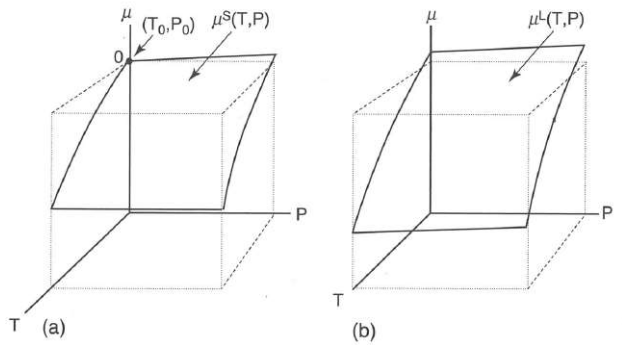
\includegraphics[width=0.55\textwidth]{Immagini/Musempl.png}
    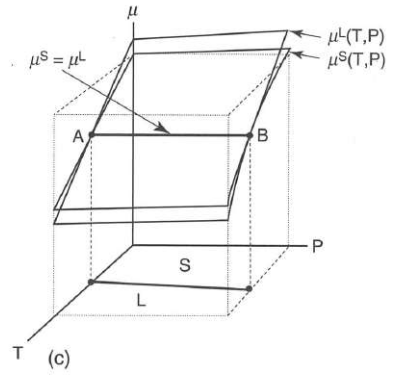
\includegraphics[width=0.35\textwidth]{Immagini/TotMu.png}
    \caption{
        Graphical rapresentation of the chemical potential for a solid phase(a), liquid phase(b) and the superposition of the two to see which one prevails on the other for the equilibrium phase(c). It's possible to see how in the part of the phase diagram where $\mu^S = \mu^L$ a coexistence line appear.
    }
    \label{fig:MuComparison}
\end{figure}

As a last remark it could be interesting to understand how the values of $\mu$ can be computed inside a system, in particular using experimental results. The idea is starting from the differential \eqref{eq:diffMu} and try to write down expressions for $S$ and $V$. To do that we need first to write down the differential of those two quantities, starting from $S$
\begin{equation}
    \label{eq:diffS}
    \dd S = \eval{\pdv{S}{P}}_T\dd P + \eval{\pdv{S}{T}}_P\dd T.
\end{equation}
We need to simplify it and the first thing that we can say is that $\mu$ is a continous function, therefore the Schwartz theorem apply having
\begin{equation}
    \pdv{\mu}{P}{T} = -\eval{\pdv{S}{P}}_{T} = \pdv{\mu}{T}{P} = \eval{\pdv{V}{T}}_P = V\alpha.
\end{equation}
Where the definition of \textbf{thermal expansion coefficient} $\alpha = V^{-1}\eval{\partial V/\partial T}_P$ was used. The remaining partial derivative in \eqref{eq:diffS} is simply the \textbf{specific heat} at constant pressure $c_P$, having so that the final form is
\begin{equation}
    \dd S = -V\alpha\dd P + \frac{c_P}{T}\dd T.
\end{equation}
Analogous considerations can be done for the volume, using also the \textbf{bulk modulus} $\beta$ having so that its final form will be instead
\begin{equation}
    \frac{\dd V}{V} = -\beta\dd P + \alpha\dd T.
\end{equation}
In this way both $V(P, T)$ and $S(P, T)$ can be computed since $\alpha, \beta$ and $c_P$ can be easily obtained experimentally and then the differential can be integrated through known numerical routines. For example, one can easily compute a so-called \textbf{isobaric section}, basically a slice of phase diagram at constant pressure $P_0$, using two consecutive integrations
\begin{align}
    &S(T, P_0) = S(T_0, P_0) + \int_{T_0}^T\frac{c_p(T')}{T'} \dd T',\\
    &\mu(T, P_0) = \mu(T_0, P_0) - \int_{T_0}^T S(T') \dd T'.
\end{align}

\subsection{Clausius-Clapeyron equation}

Now we want to completely focus on the coexistence lines and try to describe them better. In particular our main goal is to find a way to predict their form so that we will be able to draw them on the phase diagram having so, directly, all the information needed. It is renown that a solution to this is present in literature and comes with the name of \textbf{Clausius-Clapeyron equation}.
\thm{Clausius-Clapeyron equation}
{
    A coexistence line between two phases $\alpha$ and $\beta$ of a system has a slope in the $P$ vs $T$ plane that is givne by the following relation
    \begin{equation}
        \label{eq:CCequetion}
        \dv{P}{T} = \frac{1}{T}\frac{\Delta H^{\alpha \to \beta}}{\Delta V^{\alpha\to \beta}}.
    \end{equation}
}
\pf{Proof}
{
    Since we are on a coexistence line we know that the equilibrium conditions of \eqref{eq:equiCond} must be valid, therefore $\dd \mu^\alpha = \dd \mu^\beta$ along with $\dd T$ and $\dd P$, leading to
    \begin{equation}
        -S^\alpha \dd T + V^\alpha \dd P = -S^\beta \dd T + V^\beta \dd P
    \end{equation}
    Rearranging and assuming that the study is done in an isobare condition, meaning that $\dd H = T\dd S$, we will have the wanted result.
    \begin{equation}
        \dv{P}{T} = \frac{1}{T}\frac{H^\beta - H^\alpha}{V^\beta - V^\alpha} = \frac{1}{T}\frac{\Delta H^{\alpha \to \beta}}{\Delta V^{\alpha\to \beta}}.
    \end{equation}
}
\noindent
This is a really known equation that can tell us some interesting information about the system. For example, if we have the phase diagram of a transition from solid to liquid, we know that $\Delta H$ needs to be positive since the heat is transferred inside the material during melting. Therefore, if experimentally we have that the coexisting line has a positive slope, this means that the system is expanding, while its becoming smaller if the slope is negative. The latter case is something that can be clearly seen in the phase diagram of water, which is known it's a peculiar case where the volume reduce going from solid to liquid.

The equation can also be solved exactly for some simple cases of which the most important is the case of liquid-gases coexistence lines where e really simple result can be found out.
\cor{Vapor pressure curves}
{
    A coexistence line between a liquid and gases phases can be described analytically by the following equation
    \begin{equation}
        \label{eq:CCgass}
        P = c\exp\left( -\frac{\Delta H}{RT} \right),
    \end{equation}
    where $c$ is a constant.
}
\pf{Proof}
{
    We can use \eqref{eq:CCequetion} assuming that $\Delta V^{\alpha \to \beta} \approx V^{gas}$ since gases have much larger volume than liquid. Then by using the equation of perfect gas one can obtain the differential equation
    \begin{equation}
        \frac{\dd P}{P} = \frac{\Delta H}{R}\frac{\dd T}{T^2},
    \end{equation}
    where $\Delta H$ has usually a small dependence on $T$ and can therefore be assumed constant. Thus, the equation can be integrated directly giving the wanted result. 
}

\noindent
This equation allow us to describe up to a good precision the wanted lines where gasses are involved. To make an example of how good of an approximation this is we can have a look to \figref{fig:CCexample} where the coexistence lines all respect the exponential relation given by \eqref{eq:CCgass} being straight lines that changes slope on the melting point, in correspondence of a change in $\Delta H$ going from liquid-gass to solid-gass one.
\begin{figure}[t]
    \centering
    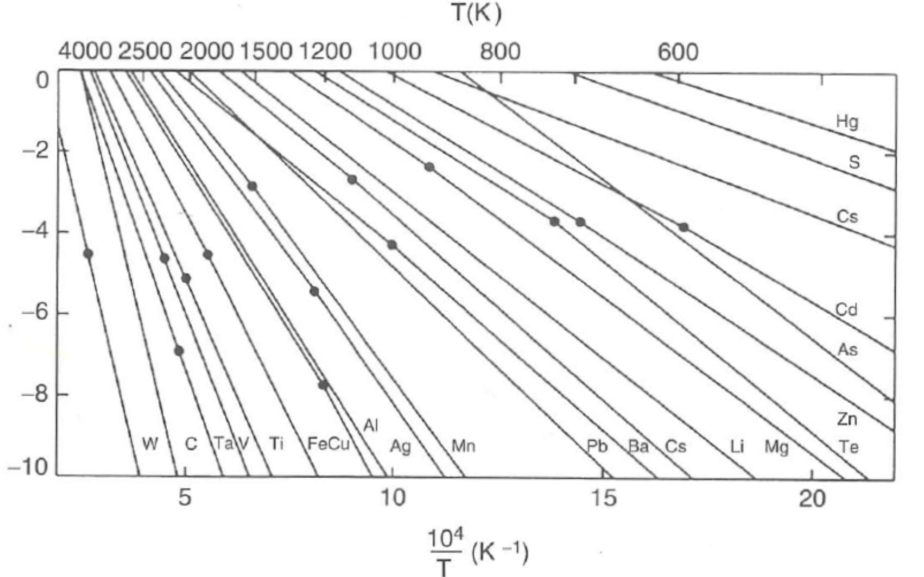
\includegraphics[width=0.6\textwidth]{Immagini/CCexample.png}
    \caption{
        Compilation of vapor pressure for the elements with $\log P$ on the y-axis. A change in slope (marked by the dot) corresponds to the melting point, which is also a triple point here because of the coexistence with the vapor phase.
    }
    \label{fig:CCexample}
\end{figure}

\nt
{
    \figref{fig:CCexample} also tells us that the difficulty in having sublimation instead melting for a material is not in the different amount of heat that we need to give in the two processes, since the slopes changes really little, but only in the needs of a much higher temperature for the former process to even start.
}